\begin{subsectionframemod}{Cross-Domain Few-Shot Object Detection}

    \metroset{block=fill}
    \begin{alertblock}{Détection d'objets few-shot cross-domain}
        Dans la détection d'objets few-shot cross-domain, on dispose de deux datasets de deux domains distincts.
        L'un est composé d'un grand nombre de données annotées (le dataset source) tandis que l'autre est plutôt limité (le dataset cible).
        L'objectif est de s'aider du dataset source pour réaliser la détection sur le dataset cible.
        Le modèle doit dans ce cas s'adapter à la fois à de nouvelles classes et à de nouvelles images ce qui complexifie la tâche.
    \end{alertblock}

    \only<1>{
        \begin{figure}
            \centering
            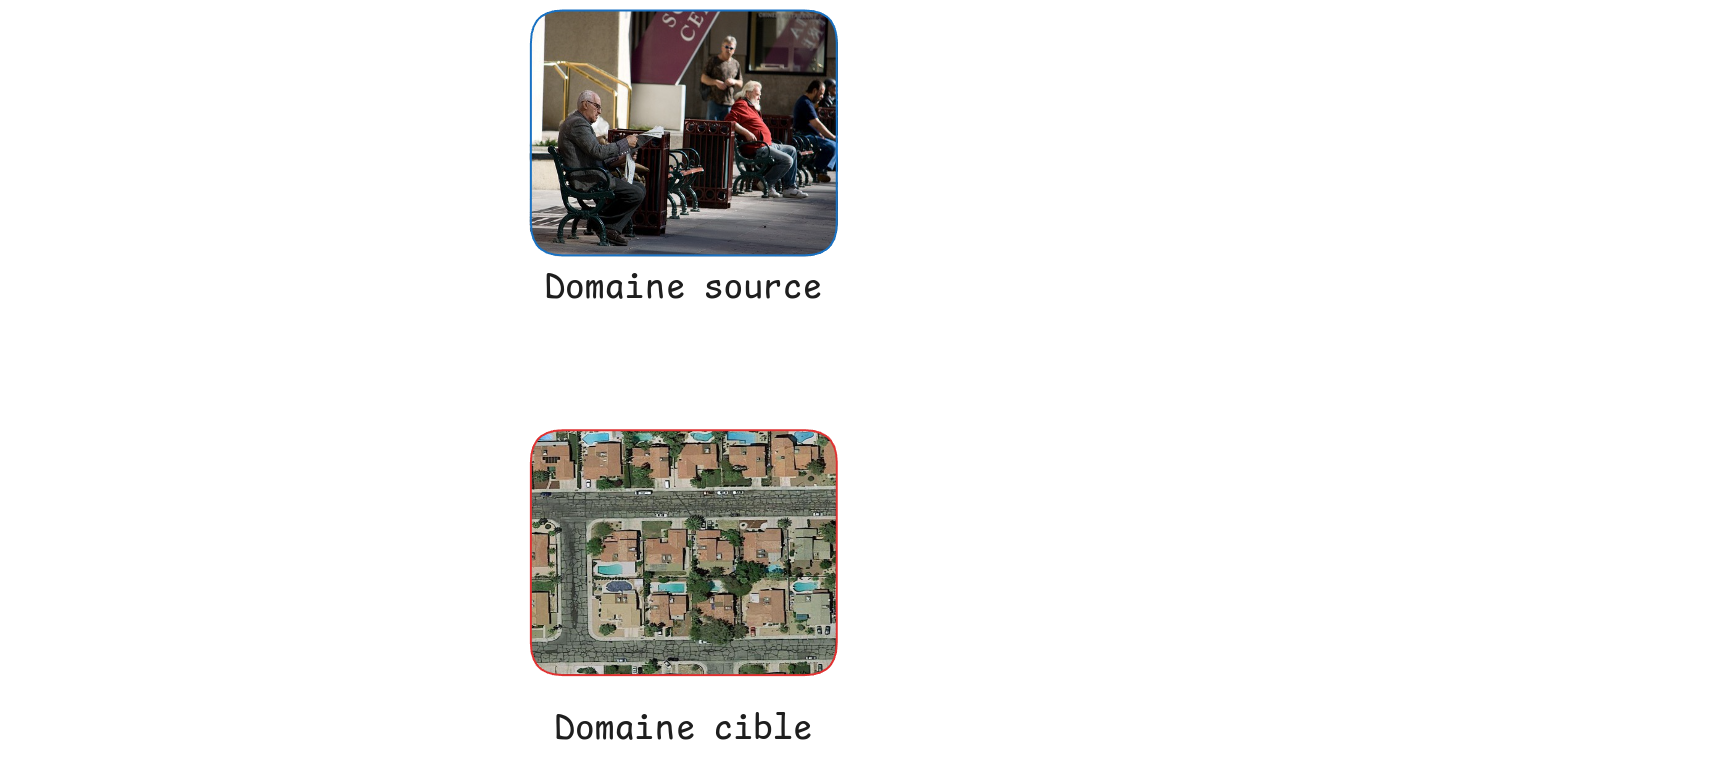
\includegraphics[width=\textwidth]{Figures/cross_domain}
        \end{figure}
    }
    \pause
    \only<2>{
        \begin{figure}
            \centering
            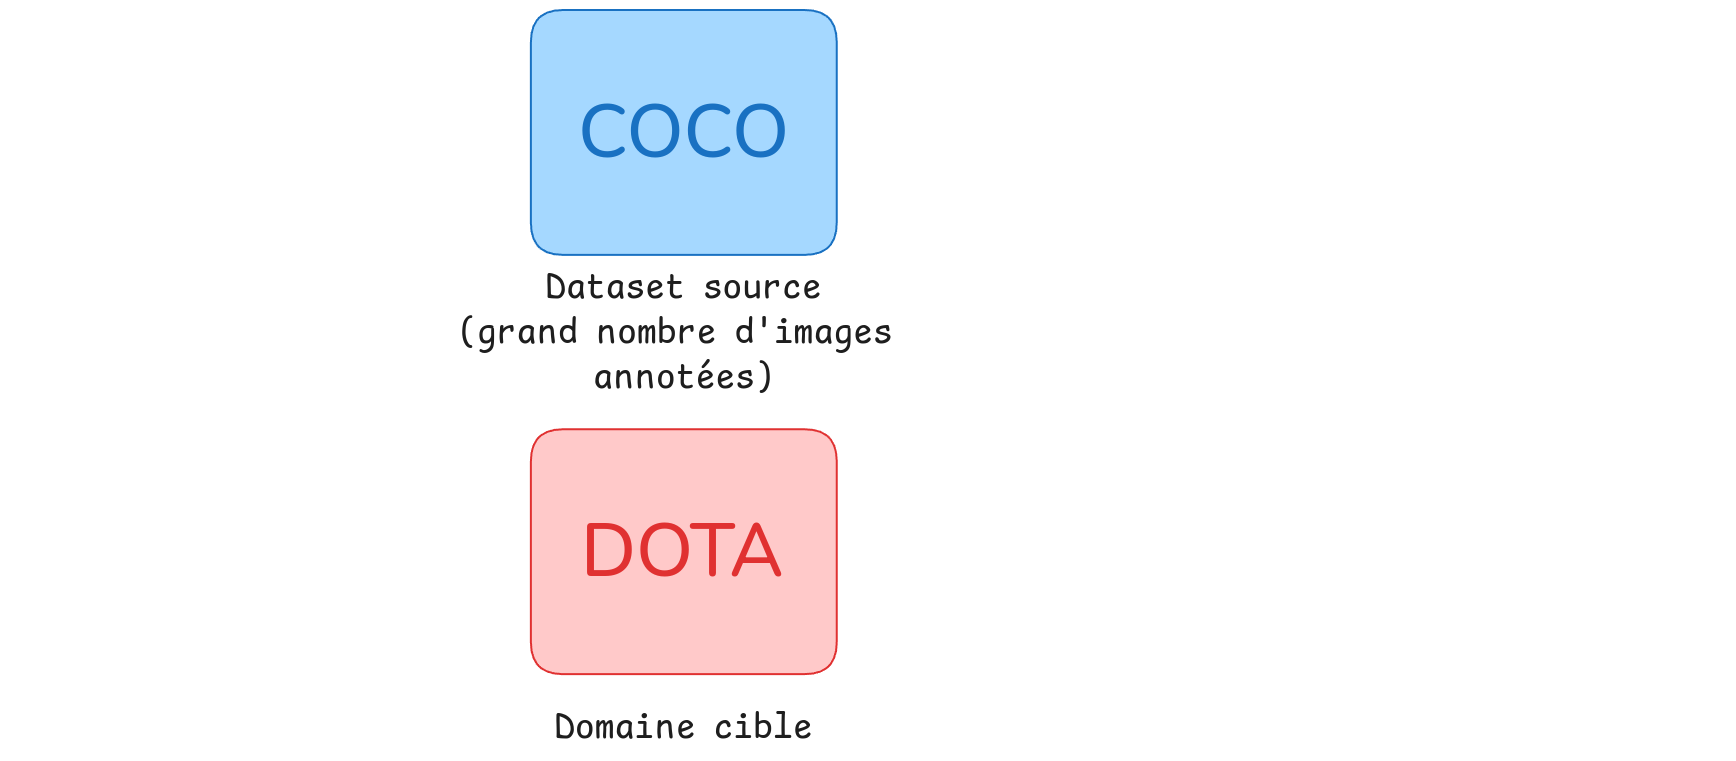
\includegraphics[width=\textwidth]{Figures/cross_domain_0}
        \end{figure}
    }
    \pause
    \only<3>{
        \begin{figure}
            \centering
            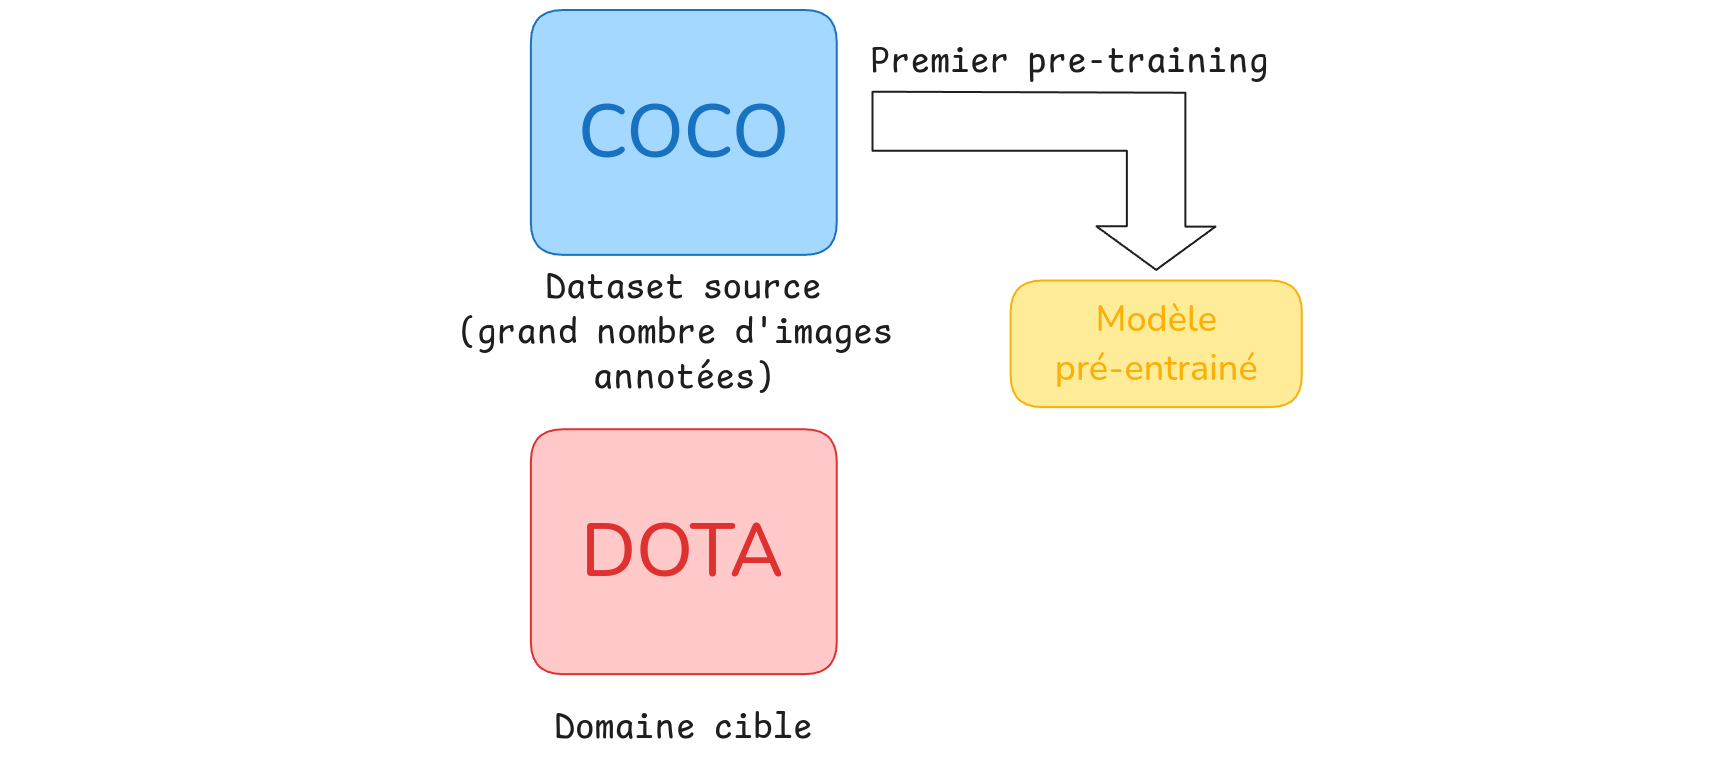
\includegraphics[width=\textwidth]{Figures/cross_domain_1}
        \end{figure}
    }
    \pause
    \only<4>{
        \begin{figure}
            \centering
            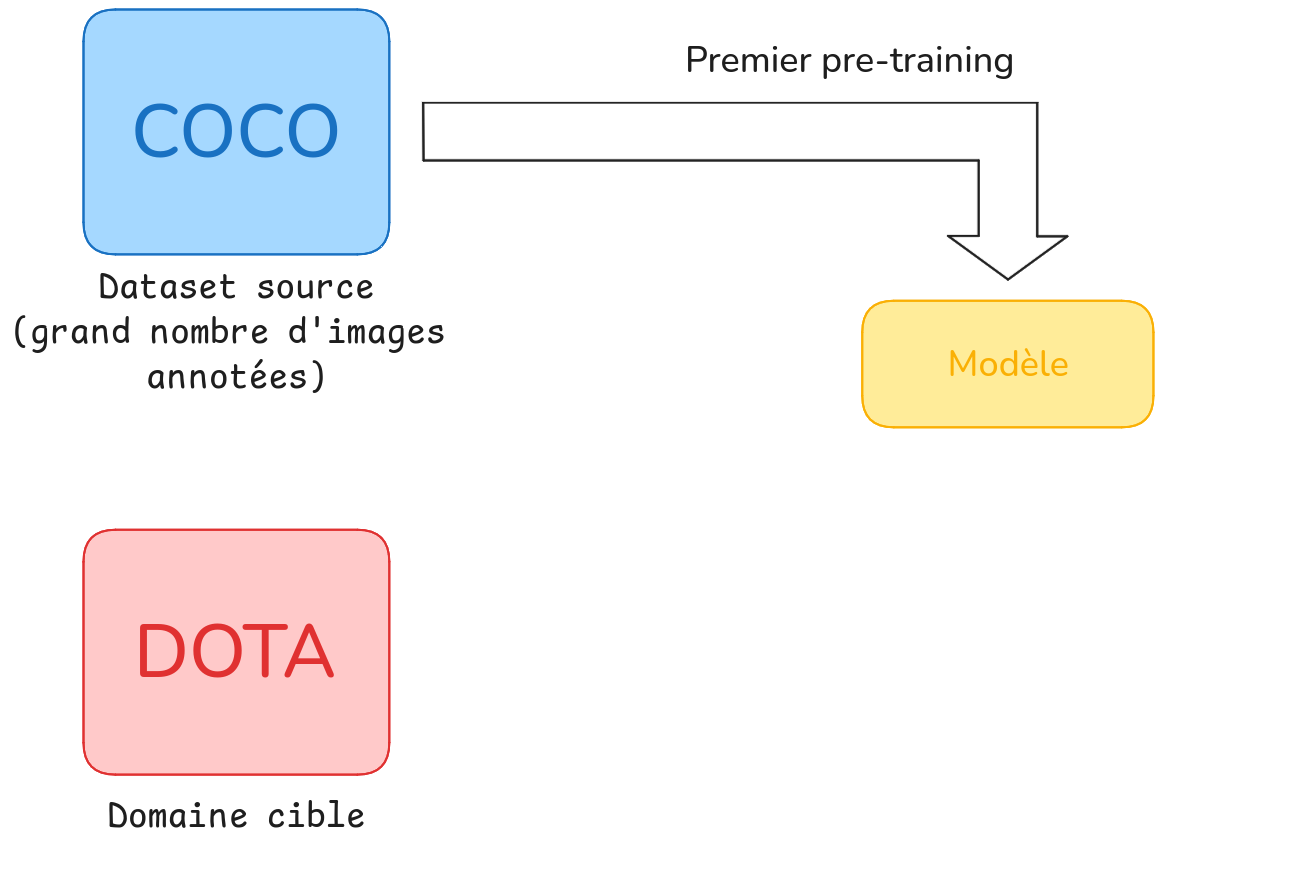
\includegraphics[width=\textwidth]{Figures/cross_domain_2}
        \end{figure}
    }
    \pause
    \only<5>{
        \begin{figure}
            \centering
            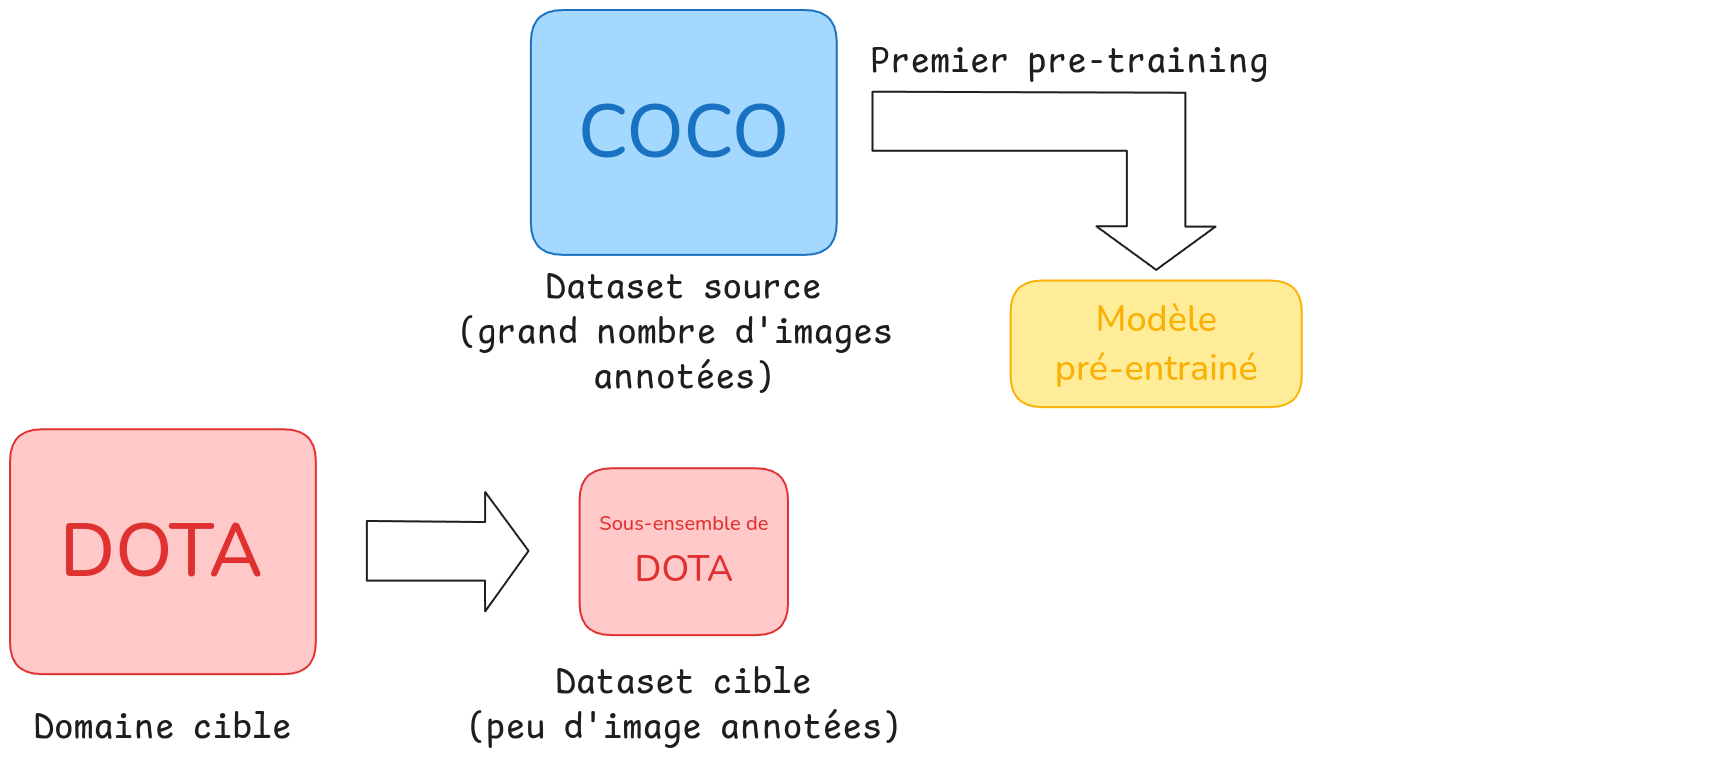
\includegraphics[width=\textwidth]{Figures/cross_domain_3}
        \end{figure}
    }
    \pause
    \only<6>{
        \begin{figure}
            \centering
            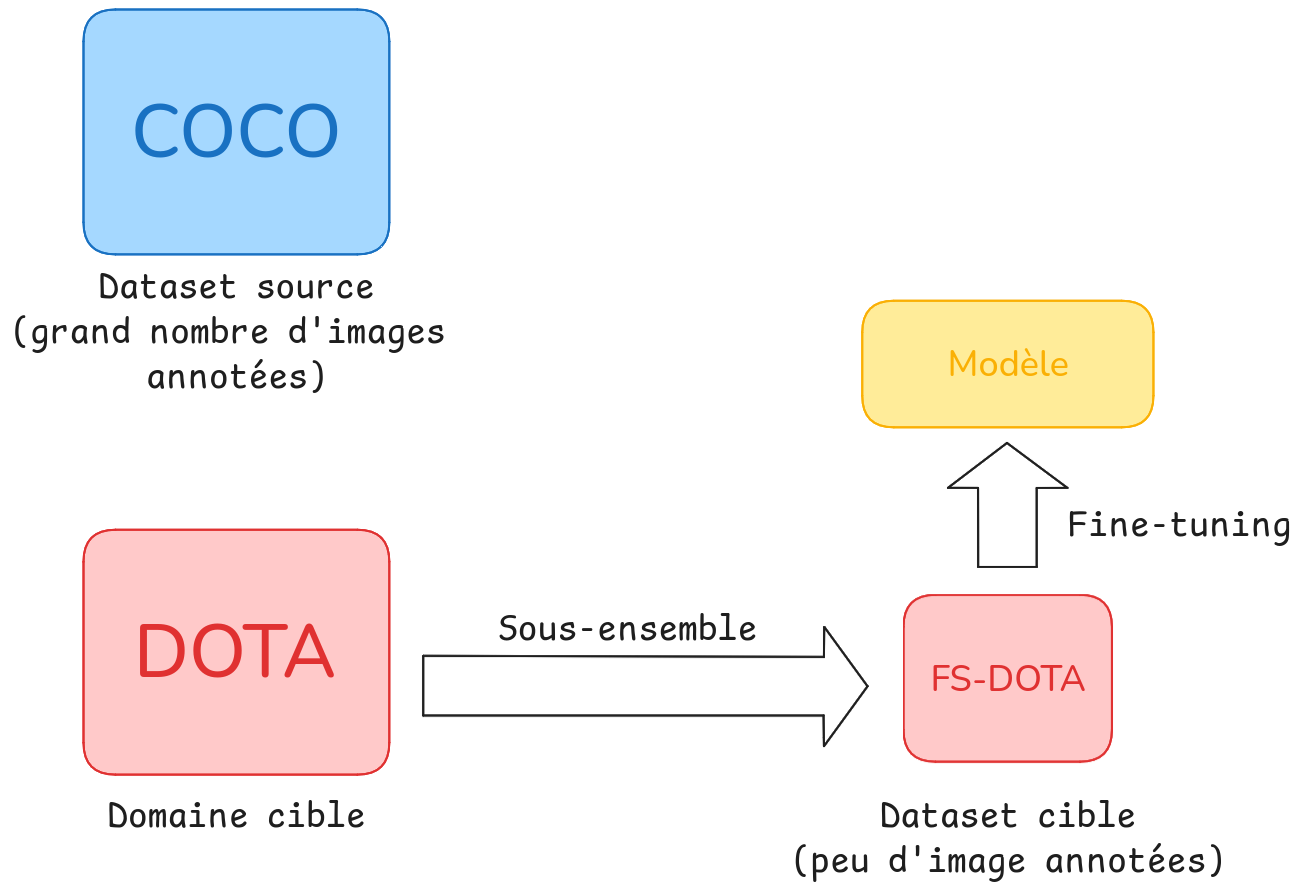
\includegraphics[width=\textwidth]{Figures/cross_domain_4}
        \end{figure}
    }

\end{subsectionframemod}